% label{eq:chap21_eq1}
\chapter{General theory of resonances and the Berggren completeness.}
\label{chap:gentheory}

\section{Physical interpretation of scattering matrix poles.}
\label{sec:physical_interpretation}  
Resonance phenomena are associated with processes taking
place in the continuum. Any quantum mechanical system may 
be experimentally found to be either in a bound stationary 
state or in a scattering state located in the positive continuum.
Resonance states with definite lifetime are never directly observed, 
but instead the scattering states into which they decay are observed. 
It is therefore natural to start with the radial Schr\"odinger equation,
for a spherically symmetric potential $V(r)$,
\begin{equation}
  \left( -{d^2\over dr^2} + v(r) + {l(l+1)\over r^2} -k^2\right) u_l(k,r) = 0
  \label{eq:chap21_eq1}
\end{equation}
here $v(r) =  2\mu V(r)/ \hbar^2  $ and the energy is related to the 
wavenumber by $k^2 =  2\mu E / \hbar^2 $, where $\mu$ is the 
reduced mass of the system. There are four different types of 
physical states associated with this Schr\"odinger equation,
bound, anti-bound, resonant and scattering states, differing in 
the boundary conditions imposed on the wave functions at large
distances. 

In the following an overview of the properties of the 
regular and irregular solutions of the Schr\"odinger equation, and
their relation to the physical scattering wave function is given. For 
a more detailed review the reader is referred to the text books 
of Newton \cite{newton} or Sitenko \cite{sitenko} on scattering theory.

Next we assume that the central potential is less singular near the origin than $r^{-2}$
and vanishes faster than $r$ at infinity, that is,
\begin{equation}
  \mathop{\lim}_{r\rightarrow 0} r^2V(r) = 0, \:\: 
  \mathop{\lim}_{r\rightarrow \infty } r V(r) = 0.
\end{equation}
From the theory of ordinary second order differential equations 
the condition that the potential $V(r)$ has a ``weaker'' singularity than $r^{-2}$� 
at the origin, means that the point $r=0$ is a \emph{regular singular point}.
It is customary to label those solutions of equation~(\ref{eq:chap21_eq1}) which 
vanish $r=0$ \emph{regular} and those which do not \emph{irregular}�
solutions. The regular $ \phi_l(k,r) $ and  irregular solutions 
$f_l(k,r)$ to equation~(\ref{eq:chap21_eq1}), are uniquely defined by 
the boundary conditions,
\begin{eqnarray}
  \nonumber
  \mathop{\lim}_{r\rightarrow 0} (2l+1)!!r^{-l-1}\phi_l(k,r) = 1, \\
  \mathop{\lim}_{r\rightarrow \infty }\exp(ikr)f_l(k,r) = i^l. 
  \label{eq:boundary}
\end{eqnarray}
The irregular solutions $f_l(k,r) $ are called the Jost solutions, and 
from the boundary condition it follows that they have the
asymptotic form 
\begin{equation}
  f_l(k,r) \rightarrow \exp(-ikr),\:\: r \rightarrow \infty
\end{equation}
The Jost solutions $f_l(k,r)$ and $f_l(-k,r)$ are linearly independent 
solutions of equation~(\ref{eq:chap21_eq1}). This follows from the 
fact that the Wronskian of $f_l(k,r)$ and $f_l(-k,r)$ is non-vanishing,
\begin{equation} 
  W\left[ f_l(k,r),f_l(-k,r)\right] = 2ik,
\end{equation}
which is easily shown using the asymptotic forms 
of the Jost solutions as $r\rightarrow \infty$. Since $f_l(k,r)$ and
$f_l(-k,r)$ are linearly independent solutions, the regular solutions 
$\phi_l(k,r) $ may be expressed as a linear combination of the Jost solutions. 
The coefficients of  $f_l(k,r)$ and $f_l(-k,r)$ are determined from 
the boundary conditions imposed on the regular solutions $\phi_l(k,r)$ at $r=0$, 
and it follows that
\begin{equation}
  \phi_l(k,r) = {1\over2} ik^{-l-1}\left[ f_l(-k)f_l(k,r) - (-1)^lf_l(k)f_l(-k,r)\right].
  \label{eq:regular}
\end{equation}
Here the Jost functions $ f_l(k) = f_l(k,r=0)$ and $ f_l(-k) = f_l(-k,r=0)$
have been introduced, and they are given by the Wronskian 
\begin{equation}
  f_l(k) = k^l W\left[ f_l(k,r),\phi_l(k,r)\right],
\end{equation}
which follows directly from equation~(\ref{eq:regular}). 
It can be shown \cite{newton, sitenko} that the regular function $\phi_l(k,r)$
is an entire function in the complex $k$-plane, while the irregular Jost solution 
$f_l(k,r)$ is an analytic function in the lower half complex $k$-plane.
From the boundary conditions in equation~(\ref{eq:boundary}) it follows 
for complex $k$ that the regular and irregular solutions satisfy the 
following conditions,
\begin{equation}
  \phi_l(k,r) = \phi_l^*(k^*,r), \:\: f_l(k,r) = f_l^*(-k^*,r). 
  \label{eq:symmetry}
\end{equation}
Further the regular solutions satisfy 
\begin{equation}
  \phi_l(k,r) = \phi_l(-k,r), 
\end{equation}
since the $\phi_l(k,r)$ is an everywhere regular function of $k^2$.

The physical scattering solutions $ u_l(k,r) $�
of equation~(\ref{eq:chap21_eq1})�are given for a mixed set
of boundary conditions, regularity at $r=0$ and the asymptotic behaviour of scattering 
wave functions as $r\rightarrow \infty$ \cite{newton}, i.e.
\begin{equation}
  u_l(k,r) \mathop{\longrightarrow}_{r\rightarrow \infty}  
  \sqrt{1\over 2\pi}i \left\{ e^{-ikr} - (-1)^l S_l(k) e^{ikr}\right\} 
  \label{eq:chap21_eq6}
\end{equation}
Here $S_l(k)$ is the partial wave scattering matrix element, which 
determines the phase shift of the outgoing wave at inifinity.
Since all physical solutions are regular at the origin, they differ from the
regular solutions $\phi_l(k,r)$ only by a normalization constant. However, 
different asymptotic behaviours of the regular solutions are specified at
specific points on the complex $k$-plane. The proper boundary 
conditions for physical states are only given at certain points in the complex $k$-plane.
If the regular solution $\phi_l(k,r)$ is
known in the entire complex $k$-plane, all physical states is in principle known.     
From equation~(\ref{eq:regular}) it follows that the asymptotic form of the regular 
solutions is given by 
\begin{equation}
  \phi_l(k,r) \mathop{\longrightarrow}_{r\rightarrow \infty} 
      {1\over2} ik^{-l-1}f_l(-k)\left\{ e^{-ikr} - (-1)^l {f_l(k)\over f_l(-k)} e^{ikr} \right\}.
\end{equation}
Comparing with equation~(\ref{eq:chap21_eq6}) it is easily seen that 
the partial wave $S$-matrix element, $S_l(k)$, is given in terms
of the Jost functions 
\begin{equation}
  S_l(k) = {f_l(k)\over f_l(-k)}.
  \label{eq:chap21_eq7}
\end{equation}
Comparing the asymptotics of the physical wave function  with the 
asymptotics of the regular solution $\phi_l(k,r)  $, 
the  physical scattering function may be written
in terms of the regular solution $\phi_l(k,r) $ and the Jost function $f_l(k)$,
\begin{equation}
  u_l(k,r) = \sqrt{2\over \pi} {k^{l+1}\phi_l(k,r)\over f_l(-k)},
  \label{eq:chap21_eq8}
  %\label{eq:chap21_eq8}
\end{equation}
which is delta-function normalized. 

Knowing all analytic properties of the Jost functions, all analytic properties 
of $S_l(k)$ follow directly.  From the definition of $S_l(k)$ given in equation~(\ref{eq:chap21_eq7})
follows that  
\begin{equation}
  S_l(-k) = S_l^{-1}(k),
  \label{eq:sym1}
\end{equation}
and from the symmetry 
property of the Jost functions given in equation~(\ref{eq:symmetry}) 
follows that
\begin{equation}
  S_l^*(k^*) = S_l^{-1}(k),
  \label{eq:sym2}
\end{equation}
where the latter property coincides with the unitarity condition for the scattering matrix 
for real values of $k$. Further, these properties establish a one-to-one correspondence 
between values of the scattering matrix in different quadrants of complex 
$k$-plane. Say that we know the value of scattering matrix at a point in the
fourth quadrant of the complex $k$-plane, $S_l(k) = {S}$. Then it
follows immediately from equation~(\ref{eq:sym1}) that $S_l(-k) = {S}^{-1}$, and 
from equation~(\ref{eq:sym2}) $ S_l(-k^*) = {S}^*$. Using again 
the symmetry relation in equation~(\ref{eq:sym1}) it finally follows
$S_l(k^*) = S_l^{-1}(-k^*)  = {S}^{-1}$. This shows that 
knowing the values of $S_l(k)$ in one quadrant of the complex $k$-plane,
the scattering matrix is automatically known in the whole complex $k$-plane.

The scattering wave function and the $S-$ matrix element $S_l(k)$ 
have poles at the same location in the complex $k$-plane, 
given by the zeroes $k = k_n$� of the Jost function $f_l(-k) = 0$. 
Due to the symmetry of the Jost functions given in equation~(\ref{eq:symmetry}), 
for each pole $k = k_n$ there is in addition a pole located at $ k = -k_n^*$. 
Furthermore the symmetry property in equation~(\ref{eq:sym1}) of $S_l(k)$ implies that for each pole $k =k_n$ 
of $S_l(k)$, it has a zero at $k=-k_n$. 
The poles in the complex $k$-plane are divided into four categories 
depending on their location in the $k$-plane, 
and are often labeled by the letters $a-d$. Consider first the case where $S_l(k)$ has
a zero for $k=-i\kappa $ for real $\kappa > 0$. Then both the regular solutions $\phi_l(k,r)$
and the physical wave functions $u_l(k,r)$ are square integrable functions since 
they fall off exponentially as $ \exp(-\kappa r)$. Furthermore the corresponding 
energy is real and negative $E = -\hbar \kappa^2/2\mu$ corresponding to a bound state
of the system. It can be shown that 
in the upper half-plane the scattering matrix $S_l(k)$ can have poles only
on the imaginary axis \cite{sitenko}. These poles correspond to the boundary conditions 
of bound states at infinity, i.e. belonging to the $\mathrm{L}^2$�functional space, with 
exponentially decaying tails, and are labeled $b$. In the lower half-plane 
the it can be shown that the poles can be positioned anywhere. 

Poles located in the fourth quadrant 
of the complex $k$-plane are associated with resonant states with outgoing 
boundary conditions at infinity, often called \emph{decaying} resonances, labeled $d$. 
To see that they correspond to outgoing asymptotics consider the regular function
in equation~(\ref{eq:regular}) at a pole of the scattering matrix,
\begin{equation}
  \phi_l(k_n,r) = \mathop{\longrightarrow}_{r\rightarrow \infty} 
      {-1\over2} (-1)^l ik^{-l-1}f_l(k_n)e^{ik_n r}
      \label{eq:asymp}
\end{equation}
A pole $k=k_n=k_1 - ik_2$ in the fourth quadrant of the
complex $k$-plane gives the specific asymptotics
\[ 
\phi_l(k_n,r) \rightarrow e ^{ik_1 r} e^{k_2 r}
\]
where $k_1,k_2 > 0$. This shows that the decay resonances correspond to outgoing 
asymptotics, furthermore they are not square integrable in the normal sense since
they are exponentially increasing and oscillating functions. 
The energy of the decay states is written in the form 
\begin{equation}
  E_n  = \mathcal{E} -i {\Gamma \over 2\mu } = 
  {\hbar^2 \over 2\mu}\left( ( k_1^2 - k_2^2) - i2k_1 k_2 \right).
  \label{eq:chap21_eq12}
\end{equation}
where the pole in the complex $k-$ plane is written 
$k_n = k_1 - ik_2$, where $k_1,k_2 > 0 $. \emph{Proper} physical resonances are 
often defined as poles where $ k_1 > k_2 $, where it is 
seen that the real part of the energy given in equation~(\ref{eq:chap21_eq12})
is positive. For poles where $k_2 > k_1$  the real part becomes negative 
and they are often called \emph{unphysical} poles.
The most interesting resonances physically, are the resonances which 
show up as sharp peaks in the cross sections, and this occurs for 
$ \Gamma \ll \mathcal{E}$. For resonance poles where the width $\Gamma $ is 
large, the resonance contribution to the cross section
tends to get smeared out within the continuum background.

For each pole located in the fourth quadrant there is a pole in the 
third quadrant symmetrically situated about the imaginary $k$- axis, these
poles corresponds to resonant states with incoming boundary conditions 
at infinity, often called \emph{capture} resonances, labeled $c$. That they are
incoming waves is seen from equation~(\ref{eq:asymp}),
\[ 
\phi_l(k_n,r) \rightarrow e ^{-ik_1 r} e^{k_2 r}, \:\:k_1 > 0,\: k_2 > 0,
 \]
Poles located on the
imaginary axis in the lower half-plane correspond to anti-bound states, labeled $a$,
often called virtual states. These states increases exponentially at large
distances, contrary to the bound states, and are clearly not normalizable, 
\[ 
\phi_l(k_n,r) \rightarrow  e^{\kappa r}, \:\: \kappa > 0.
 \]
Figure~\ref{fig:smat_poles} sums up the most general distribution of poles 
of the scattering matrix and the corresponding zeros.
\begin{figure}[hbtp]
\begin{center}
\resizebox{12cm}{10cm}{\epsfig{file=figures/smat_poles.eps}}
\end{center}
\caption{Distribution of $S-$ matrix poles (filled circles) and corresponding
  zeroes (open circles) in the complex $k-$plane. $a =$ anti-bound, 
 $ b = $ bound, $c = $ capture and $d =$ decay.}  
\label{fig:smat_poles}
\end{figure}

\section{Regularizing divergent integrals of states on the second energy sheet.}
\label{sec:divergent_integrals}
The radial wave function $u_l(k,r)$ of a decay 
resonant state, with $k = k_n$ located in the fourth quadrant of the complex
$k-$plane, satisfies the radial Schr\"odinger equation ~(\ref{eq:chap21_eq1}).
The decay resonances are regular at the origin, $ u_l(k,0) = 0$, 
and have purely outgoing waves, $u_l(k,r) \rightarrow O_l(k,r)$, at infinity 
as  boundary conditions. 
If the potential has a finite range, in the sense
that it vanishes identically beyond some finite distance $r=a$. The outgoing
solutions $O_l(kr)$ 
are given in terms of spherical Riccati-Hankel functions $h_l^{(+)}(kr)$.
In the case of long-range potentials, such as the Coulomb potential, 
the asymptotic form of the wave functions are given by the  more complicated
Coulomb functions.

From the requirement that the wave functions and their derivatives should be
continuous at the boundary of the potential $r=a$, follows that the logarithmic 
derivative should be continuous, giving the condition
\begin{equation}
  u_l(k,a){O'}_l(k,a) - {u'}_l(k,a)O_l(k,a) = 0.
\end{equation}
For each pole $k=k_n$ in the fourth 
quadrant there is a pole $k=\tilde{k}_n=-k_n^*$ in the third quadrant 
associated with a capture resonance. The capture
states, $ u_l(\tilde{k}_n,r)$, 
are solutions of the complex conjugated version of 
the radial Schr\"odinger equation (\ref{eq:chap21_eq1}), with  regularity at the 
origin and with purely incoming waves at infinity, $I_l(k,r)$. 
Where $I_l(kr)$ 
is given in terms of spherical Riccati-Hankel functions $h_l^{(-)}(kr)$.
The corresponding boundary conditions for the capture states becomes, 
\begin{equation}
  {u}_l(\tilde{k},a){I'}_l(\tilde{k},a) - {{u}'}_l(\tilde{k},a)I_l(\tilde{k},a) = 0.
\end{equation}
In the following we define the the decay and capture states by
\begin{equation} 
  u_{nl}(r) \equiv u_l(k_n,r), \:\: \tilde{u}_{nl}(r) \equiv u_l(\tilde{k}_n,r) 
\end{equation}
The capture and decay resonances are related through 
\begin{equation} 
  \tilde{u}_{nl}(r) = u_{nl}^*(r), \:\: \mathrm{i.e.} \:\: \tilde{u}_{nl}^*(r) = u_l(r)
\end{equation}
Normalization of the decay resonances through the usual Euclidean inner product, 
\begin{equation}
  \langle {u}_{nl} \vert u_{nl}\rangle=
  \int_0^\infty dr\: u_{nl}^*(r)u_{nl}(r) = 
  \int_0^\infty \tilde{u}_{nl}(r)u_{nl}(r) 
\end{equation}
is not possible in the upper limit, since the integrand diverges exponentially as 
\begin{equation}
  \tilde{u}_{nl}(r)u_{nl}(r) \mathop{\longrightarrow}_{r\rightarrow\infty} 
  e^{2 k_2 r}
\end{equation}
for $k_n = k_1 -ik_2 $ and $k_1,k_2 > 0 $.
On the other hand, the fact the decay and capture resonances come in conjugate pairs,
may suggest that they form a \emph{bi-orthogonal} set 
of functions, and that the normalization integral,
\begin{equation}
  \langle \tilde{u}_{nl} \vert u_{nl}\rangle = \int_0^\infty \tilde{u}_{nl}^*(r)u_{nl}(r) = 
  \int_0^\infty u_{nl}^2(r), 
\end{equation}
may exist, and be given a definite value.
The integrand of this integral still increases exponentially but 
oscillates as 
\begin{equation}
  \tilde{u}_{nl}^*(r)u_{nl}(r) \mathop{\longrightarrow}_{r\rightarrow\infty} 
  e^{ 2ir \left( k_1 -ik_2\right) }.
  \label{eq:eq220}
  %\label{eq:eq220}
\end{equation}
The hope is that the oscillations at large distances will cancel each other, 
such that 
\begin{equation}
  0 < \vert \langle \tilde{u}_l(k) \vert u_l(k)\rangle \vert < \infty
\end{equation}

\subsection{Regularization by $e^{-\epsilon r^2}$.}

From the theory of divergent integrals and series, see e.g. Ref.~\cite{hardy}, 
many integrals which are divergent in the conventional sense, may be regularized by some
regularization procedure. Zel'dovich \cite{zeldovich} proposed the following 
integration procedure for regularizing integrals involving resonant states,
which have an exponentially oscillating divergent tail along the real $r$-axis. 
\begin{equation}
  I = \mathop{\lim}_{\epsilon \rightarrow 0}\int_0^\infty dr\:e^{-\epsilon r^2}u_{nl}^2(r)
  \label{eq:norm_int}
\end{equation}
From the asymptotic behaviour of the resonant states in equation~(\ref{eq:eq220}), it 
is natural to study the integral 
\begin{equation}
  I_n(k) = \mathop{\lim}_{\epsilon \rightarrow 0} I_n(k,\epsilon) = 
  \mathop{\lim}_{\epsilon \rightarrow 0}\int_0^\infty dr\:e^{-\epsilon r^2}r^n e^{\kappa r} ,
\end{equation}
where $n = 0,1 $ and $ \kappa = i k$. For a positive and finite value $\epsilon$ 
the regularizing factor $e^{-\epsilon r^2}$ decreases more rapidly than the 
exponential function  $ e^{\kappa r}$ increases for an arbitrary exponent $\kappa$, and 
the integral �$I_n(k,\epsilon)$ converges. It is convienient to introduce a variable
change in $I_0(k,\epsilon)$
\begin{equation}
  t = r\sqrt{\epsilon}, \:\: x = {\kappa \over 2 \sqrt{\epsilon}} 
\end{equation}
which gives
\begin{equation}
  I_0(k,\epsilon) = {1\over \sqrt{\epsilon}}e^{x^2}\int_{-x}^\infty dt\: e^{-t^2} = 
  \sqrt{ { \pi\over \epsilon}}e^{x^2}\left[ 1 - 2\mathrm{Erfc}(x)\right]
\end{equation}
where 
\begin{equation}
  \mathrm{Erfc}(x) = {2\over \sqrt{\pi}}\int_x^\infty dt\: e^{-t^2}.
\end{equation}
is the complementary error function \cite{boas}. As $\epsilon \rightarrow 0 $ 
then $ x \rightarrow \infty $, and using the asymptotic expansion of the error function \cite{boas}, the
integral $I_0(k,\epsilon) $ may be written as 
\begin{eqnarray}
  \nonumber
  I_0(k,\epsilon) & = & \sqrt{\pi \over \epsilon}e^{x^2} - 
  {1\over 2x\sqrt{\epsilon}}\left( 1 - {1\over 2x^2} + {3\over 4x^4} - ...\right)  \\  
  & = & \sqrt{\pi \over \epsilon}e^{-{k^2\over 4\epsilon}} + {i\over k} -{2\epsilon \over k^3} + O(\epsilon^2).
  \label{eq:eq227}
  %\label{eq:asymp2}
\end{eqnarray} 
The integral $I_1(k,\epsilon)$ is calculated using the relation,
\begin{equation}
  I_1(k,\epsilon) = {\partial \over \partial \kappa} I_0(k,\epsilon) = 
  {1\over 2\epsilon}\left( \kappa I_0(k,\epsilon) +1 \right),  
\end{equation} 
Inserting the asymptotic expansion for $I_0(k,\epsilon)$ in equation~(\ref{eq:eq227}), 
gives for the $I_1(k,\epsilon)$ integral,
\begin{equation}
  I_1(k,\epsilon) = -\sqrt{ \pi \over 4\epsilon^3 }ike^{-{k^2\over 4\epsilon} } - {1\over k^2} + O(\epsilon).
\end{equation}  
Dealing with regularization of integrals involving \emph{proper} resonances, 
in which the real part of the resonance energy is positive,
the restriction  $\vert \mathrm{Re}\:k\vert > \vert \mathrm{Im}\:k \vert $ follows, and 
consequently $ \mathrm{Re}\:k^2 > 0$.�In this case the relation 
\begin{equation}
  \mathop{\lim}_{\epsilon \rightarrow 0} \epsilon^p e^{ -{k^2 \over 4\epsilon} } = 0,
 \end{equation}
is valid for any real $p$, and may be used to obtain the following 
finite expressions for the integrals $I_0(k)$ and $I_1(k)$,
\begin{equation}
  I_0(k) = { i\over k}, \:\: I_1(k) = -{1 \over k^2}.
\end{equation}

\subsection{Regularization by complex scaling.}
The regularization factor $e^{-\epsilon r^2}�$ is not unique, and there exists 
a variety of other regularization procedures,  all yielding the same unique finite
result for the integrals $I_1(k)$ and $I_2(k)$. One such regularization procedure,
more tractable from a numerical standpoint, is based on complex rotation in the complex
$r$-plane, first discussed in Ref.~\cite{gyarmati}.
Consider the zero contour integrals 
\begin{equation}
  \int_C dz\: e^{ik z} = 0, \:\:  \int_C dz\: z e^{ik z} = 0,
 \end{equation}
where the contour $C=C_1 + C_2 + C_3 $ is defined by a rotation angle $\theta$ 
in the complex $r$-plane as shown in figure~\ref{fig:rcontour}.  
\begin{figure}[hbtp]
\begin{center}
\resizebox{10cm}{8cm}{\epsfig{file=figures/rcontour.eps}}
\end{center}
\caption{Integration contour in the complex�$r$-plane used for
  regularization of integrals involving resonant states.}
\label{fig:rcontour}
\end{figure}
For $R\rightarrow \infty $ the integral along the arc $C_2$ vanishes and 
by the Cauchy Riemann integral theorem it follows 
\begin{eqnarray}
  \tilde{I}_0(k) = \int_0^\infty dr\: e^{ik r} 
  = e^{i\theta} \int_0^\infty  dr\: e^{ik r \left( \cos\theta + i\sin\theta\right)} \\
  \tilde{I}_1(k) = \int_0^\infty dr\: r e^{ik r} 
  = e^{2 i\theta} \int_0^\infty  dr\: r e^{ik r \left( \cos\theta + i\sin\theta\right)}. \\
\end{eqnarray}
For $k = k_1 - ik_2$ and $k_1,k_2 > 0$ these integrals converge for a rotation angle 
$ \theta > \mathrm{atan}( k_2/k_1) $, and it is easily shown that they take the finite
values
\begin{equation}
  \tilde{I}_0(k) = {I}_0(k) = {i\over k},
\end{equation}
In the same way it is easily shown that 
the integral $\tilde{I}_2(k)$ takes the finite value
\begin{equation}
  \tilde{I}_1(k) = {I}_1(k) = -{1\over k^2},
\end{equation}
illustrating that different regularization procedures of divergent integrals 
must yield the same unique finite value, if it exists.

From the above 
analysis it is found that the innerproduct given in equation~(\ref{eq:norm_int})
of a $d$ - and the corresponding conjugate $c$ resonant state 
may be given a finite value, i.e. it is possible to normalize these states.
It remains to examine whether resonant states at different energies, i.e. 
$k_1 \neq k_2$, form a \emph{bi-orthogonal} set. Starting with the Schr\"odinger equation 
for two different resonant states $u_{n_1l}(r)$ and $ u_{n_2l}(r)$ and multiplying the 
left with $u_{n_2l}(r)$ and $ u_{n_1l}(r)$ respectively, one obtains by subtracting the 
two equations,
\begin{equation}
  {d\over dr}\left[ u_{n_2l}(r)u'_{n_1l}(r) - u'_{n_2l}(r)u_{n_1l}(r)\right] = 
  \left( k_2^2 -k_1^2 \right) \tilde{u}_{n_2l}^*(r)u_{n_1l}(r).
 \end{equation}
Multipying from the left with $\int_0^\infty dr\: e^{-\epsilon r^2}$, 
one obtains the following expression by partial integration,
\begin{eqnarray}
  \nonumber
  \int_0^\infty dr\: e^{-\epsilon r^2} {d\over dr}\left[ u_{n_2l}(r)u'_{n_1l}(r) - u'_{n_2l}(r)u_{n_1l}(r)\right]  = \\
  \nonumber
  2\epsilon \int_0^\infty dr\: r e^{-\epsilon r^2}\left[ u_{n_2l}(r)u'_{n_1l}(r) - u'_{n_2l}(r)u_{n_1l}(r)\right]  \\
  = \left( k_2^2 - k_1^2 \right)\int_0^\infty dr\: e^{-\epsilon r^2}\tilde{u}_{n_2l}^*(r)u_{n_1l}(r), 
  \label{eq:eq239}
  %\label{eq:norm_int2}
\end{eqnarray}
where the boundary condition $u_{nl}(r=0) = 0$ has been used. 
From the asymptotic form of the integrand 
$ r e^{-\epsilon r^2}�e^{i(k_1 + k_2)r} $  it is seen that the integrals in equation~(\ref{eq:eq239})
are comparable with the finite result for the integral $I_1(k,\epsilon)$
as $\epsilon \rightarrow 0$. It follows that 
\begin{equation}
  \left( k_2^2 - k_1^2 \right)\mathop{\lim}_{\epsilon \rightarrow 0} 
  \int_0^\infty dr\: e^{-\epsilon r^2}\tilde{u}_{n_2l}^*(r)u_{n_1l}(r) = 0. 
\end{equation}
Defining the inner product of resonant states as this limit, we finally obtain 
\begin{equation}
  \langle \tilde{u}_{n_1l} \vert u_{n_2l} \rangle = 
  \langle {u}_{n_1l}^* \vert u_{n_2l} \rangle = \delta_{n_1,n_2},
  \label{eq:eq241}
  %\label{eq:cproduct}
\end{equation}
which shows that the resonant states together with the bound states
are orthogonal in this sense. In the case where bound states enter the 
inner product, there is no divergence problem since the bound states 
has an exponential decay as $r\rightarrow \infty$.
This symmetric inner product is often called the $c$- product \cite{nimrod}, 
which states that the resonances form a \emph{bi-orthogonal} set. In the case where 
$k_1$ and $k_2$ are real, the $c$-product coincides with the usual Hermitian inner product.

 
\section{The generalized Berggren completeness; proof and discussion}
\label{sec:berggren}
We have shown that the regular solution $\phi_l(k,r)$ with 
$k=k_n$ being the poles of the scattering matrix or zeros of the Jost function, can 
be normalized by some regularization procedure. Further it was shown that
regular solutions $\phi_l(k,r)$ located at different $k_n$ 
in the complex $k$-plane are orthogonal to each other, 
through the symmetric inner product given in equation~(\ref{eq:eq241}). This 
suggests that the regular solutions at the 
poles of the scattering matrix, are part of a complete set of 
\emph{bi-orthogonal}�states, which may serve as an expansion basis 
when dealing with processes taking place in the continuum regime. This is the
subject of this section. 

We start with the standard completeness relation 
defined along the real $k$-axis, 
\begin{equation}
  \sum_{n=b} u_{ln}(r)u_{nl}^*(r')\vert + 
      {1\over 2}�\int_{-\infty}^\infty dk\: u_l(k,r) u_l^*(k^*,r') = \delta(r-r')
      \label{eq:eq242}
\end{equation}
where the discrete sum is over the bound state poles located along the 
positive imaginary $k$-axis, and the integral is over the continuum of 
scattering functions located along the real $k$-axis. Note that on the real axis 
we have $u_l^*(k^*,r') = u_l^*(k,r') $.
A proof of this completeness is given by Newton in Ref.~\cite{newton}. Newton considered 
the integral 
\begin{equation}
  I(r) = \int_C dk\:k\int_0^\infty d{r'}\: h(r')G_l(k;r,r'),
  \label{eq:eq243}
  %kanskje litt mere utfyllende om Newtons bevis...
\end{equation}
where $h(r)$ is part of the L$^2$ functional space and $G_l(k;r,r')$ is 
the complete Green's function or resolvent. The integration contour 
$C$�
runs along the real $k$-axis from $-\infty $ to $\infty $, and is closed 
by a semicircle in the upper half $k$-plane. The Green's function has 
poles at the same locations in the complex $k$-plane as the 
scattering matrix, and using Cauchy's residue theorem the various contributions 
to the integral in equation~(\ref{eq:eq243}) is evaluated by the residues at the
bound state poles along the positive imaginary $k$-axis. In the end it is 
shown that a $l^2$ function $h(r)$ may be expanded in a complete
set of bound- and scattering wave functions given in equation(\ref{eq:eq242}).
The class of square integrable functions, includes those with 
exponential asymptotics, $ h(r) \rightarrow e^{ikr}, \: r \rightarrow \infty $, 
where $k$ is in the upper half complex $k$-plane.  

\begin{figure}[hbtp]
\begin{center}
\resizebox{12cm}{9cm}{\epsfig{file=figures/int_contour1.eps}}
\end{center}
\caption{Integration contour $C = L +S$ used in deriving the Berggren completeness relation.}
\label{fig:int_contour1}
\end{figure}
In Ref.~\cite{berggren} Berggren showed that there exist 
a modified completeness relation, where the resonant contributions hidden in the
continuum integral were disentangled from the background of continuum states, 
and included in the discrete sum over bound states.
The proof of Berggren, is based on the same complex analysis used by Newton,  
only that the integration contour $C$ in equation~(\ref{eq:eq243}) where modified to enclose not
only the bound state poles, but in addition a set of \emph{proper}�
resonant poles, 
see figure~\ref{fig:int_contour1}.

Later Lind \cite{lind} presented a straightforward method for deriving 
various completeness relations starting from the standard 
completeness relation given in equation~(\ref{eq:eq242}). 
This method is based on analytic 
continuation of the integral over scattering functions, using the 
the known analytic properties of the scattering functions in the complex
$k$-plane. As discussed in the previous section \ref{sec:physical_interpretation}, the
scattering functions have poles wherever the Green's function $G_l(k)$ or the scattering matrix 
elements $S_l(k)$ have poles. Deforming the integration contour defined
along the real $k$-axis for the continuum integral in equation~(\ref{eq:eq242}), one obtains 
by the Cauchy residue theorem
\begin{equation}
  �-\int_{0}^\infty dk\: u_l(k,r) \tilde{u}_l^*(k,r') + 
   \int_{L^+} dk\: u_l(k,r) \tilde{u}^*_l(k,r') = 
   2\pi i \sum_{k_n \in  {\bf C}} \mathop{\mathrm{Res}}_{k = k_n} u_l(k,r) \tilde{u}^*_l(k,r'),
   %\label{eq:int_contour2}
   \label{eq:eq244}
\end{equation}
where the contour $L^+$ is part of the inversion symmetric contour $L = L^- +L^+$, and is
the deformation of the positive real $k$-axis. Here $\tilde{u}_l(k,r) = u_l(k^*,r)$ are associated 
with scattering functions on the conjugated contour $L^*$,  which  encloses the capture 
resonances which are orthogonal to the decay resonances enclosed by $L$. 
Inversion symmetric contour meaning that if $k$ is on $L$, then so is $-k$. 
The product of scattering functions $ u_l(k,r) \tilde{u}_l(k,r') $ is a meromorphic function of
$k$ with poles given by the Jost functions $f_l(-k) = 0 $ and  $f_l^*(-k^*) =0 $.
The residue is evaluated 
at each pole $k=k_n$ of the scattering functions, 
located in the region between the contour $L^+$ and 
the real positive $k$-axis labeled ${\bf C}$.
In writing equation~(\ref{eq:eq244}) the inversion symmetry of $L$ and the 
symmetry of the integrand in the continuum integral has been exploited to give
\begin{equation}
  \int_{L^-} dk\: u_l(k,r)  \tilde{u}_l^*(k,r') = 
  \int_{L^+} dk\: u_l(k,r)  \tilde{u}_l^*(k,r')
\end{equation}
In Ref.~\cite{lind} the importance of choosing an inversion symmetric contour was discussed. If $L$ is 
inversion symmetric, the complex continuum integral can be rewritten in terms of scattering functions,
and the continuum integrals can be written using energy as the integration variable.
In deriving the general Berggren completeness the residues in equation~(\ref{eq:eq244}) 
have to be evaluated. Writing the physical wave function in terms of the 
regular solution and the Jost  function, see Sec.~\ref{sec:physical_interpretation}
for further details, one gets
\begin{equation}
  u_l(k,r) = \sqrt{2\over \pi} {k^{l+1}\phi_l(k,r)\over f_l(-k)},
\end{equation}
and for the conjugate wave function $\tilde{u}_l(k,r)$,
\begin{equation}
  \tilde{u}_l(k,r) = u_l(k^*,r) = \sqrt{2\over \pi} {(k^*)^{l+1}\phi_l(k^*,r)\over f_l(-k^*)} = 
  \left(  \sqrt{2\over \pi} {k^{l+1}\phi_l(k,r)\over f_l(k)} \right)^*,
\end{equation}
where use has been made of the symmetry properties of the regular and Jost functions
given in equation~(\ref{eq:symmetry}). The residue in equation~(\ref{eq:eq244}) may then 
be written as
\begin{equation}
  \mathop{\mathrm{Res}}_{k = k_n} u_l(k,r) \tilde{u}_l^*(k,r') = 
  \mathop{\mathrm{Res}}_{k = k_n} {2\over \pi} {k^{2l+2}\phi_l(k,r)\phi_l(k,r')\over f_l(k)f_l(-k)},
  \label{eq:residue}
\end{equation}
Making use of the property $\mathop{\mathrm{Res}}_{z = z_0} h(z)/g(z) = h(z_0)/g'(z_0) $ 
where $h(z)$ and $g(z)$ are analytic functions at $z=z_0$, it is seen that following 
derivative has to be evaluated, 
\begin{equation}
\left. {d\over dk} f_l(k)f_l(-k) \right| _{k=k_n} = 
 f_l(k_n) \left. {d\over dk}f_l(-k)\right| _{k=k_n},
\end{equation}
here the fact the Jost function $f_l(-k) = 0 $ for $k=k_n$  has been used. 
The problem of determining the residue in equation~(\ref{eq:eq244}) has now been reduced to 
the problem of determining the derivative of the Jost function at the resonance pole $k=k_n$.
In Ref.~\cite{lind} the derivative of the Jost function where proven to be 
\begin{equation}
 \left. {d\over dk}f_l(-k)\right| _{k=k_n} = i4k_n^{2l+2} Reg \int_0^{\infty} dr r^2\phi^2_l(k_n,r) = 
 i4k_n^{2l+2}N^2,
\end{equation}
where $N$ is the norm of the regularized resonances wave functions appearing in the integral. 
The sum over residues in equation~(\ref{eq:eq244}) now becomes, 
\begin{eqnarray}
\nonumber
  2\pi i \sum_{k_n \in {\bf C}} \mathop{\mathrm{Res}}_{k = k_n} u_l(k,r) \tilde{u}^*_l(k,r') = 
  4i \sum_{k_n \in {\bf C}}  {k^{2l+2}\phi_l(k_n,r)\phi_l(k_n,r')\over 
    \left. {d\over dk} f_l(k)f_l(-k)\right|_{k=k_n}} \\ 
  = \sum_{k_n \in {\bf C}} {\phi_l(k_n,r)\phi_l(k_n,r')\over N^2} = \sum_{k_n \in {\bf C}} u_{nl}(r)\tilde{u}_{nl}^*(r'),
\end{eqnarray}
inserting this into equation~(\ref{eq:eq244}), one gets the following expression for 
the integral over scattering functions along the real $k$-axis (positive energy states),  
\begin{equation}
  �\int_{0}^\infty dk\: u_l(k,r)  \tilde{u}_l^*(k,r') = 
   \sum_{k_n \in  {\bf C}} u_{nl}(r) \tilde{u}_{nl}^*(r') + 
   \int_{L^+} dk\: u_l(k,r)  \tilde{u}_l^*(k,r'),
\end{equation}
where it is explicitly seen that the resonant contributions hidden in the the continuum 
integral along the real $k$-axis has been disentangled. In Ref.~\cite{lind} it was shown 
for finite range potentials that the continuum integral along the contour $L^+$ produces
a smooth background, but is in most cases non-neglible. Switching to abstract vector notation,
it has been shown that for a general inversion symmetric 
contour $L$, see figure~\ref{fig:int_contour2}, the generalized Berggren 
completeness becomes, 
\begin{equation}
  {\bf 1} = \sum_{n= a,b,c,d} \vert u_{nl}\rangle \langle \tilde{u}_{nl}\vert + 
  �\int_{L^+} dk\:\vert u_l(k) \rangle \langle \tilde{u}_l(k)\vert.  
   %\label{eq:berggren}
   \label{eq:eq248}
\end{equation}
The discrete sum includes all types of poles of the scattering matrix, i.e.
anti-bound (a), bound (b), capture resonant (c) and decay resonant (d) states. This 
completeness can be used to expand all functions with exponential asymptotics,  
$e^{ikr}, \: r \rightarrow \infty �$ where $k$ is located within the closed
contour $C= L+S$. Keeping only the discrete part of the completeness 
relation (\ref{eq:eq248}), one ends up with the pole-approximation.   
\begin{figure}[hbtp]
\begin{center}
\resizebox{12cm}{9cm}{\epsfig{file=figures/int_contour2.eps}}
\end{center}
\caption{General inversion symmetric contour $C = L +S$ used in deriving the 
  generalized Berggren completeness relation. The black circles represents the poles which 
  are included in the discrete sum, while the red circles are poles which are embedded in the 
  continuum integral along the contour $L^+$.} 
\label{fig:int_contour2}
\end{figure}
As shown in figure~\ref{fig:int_contour2} a typical inversion symmetric 
contour cannot separate all poles from the continuum integral. In this particular case
the red circles gives the poles which are not included in the discrete sum, while
the black circles give the poles which are included in the sum. It is important to emphasize 
that completeness defined either along the real $k$-axis or along a distorted contour $L$ in 
the complex $k$-plane are equivalent in the sense, 
\begin{eqnarray}
  \nonumber
      {\bf 1} & = & \sum_{n= a,b,c,d} \vert u_{nl}\rangle \langle \tilde{u}_{nl}\vert + 
      �\int_{L^+} dk\:\vert u_l(k) \rangle \langle \tilde{u}_l(k)\vert \\
       & = &  \sum_{n= b} \vert u_{nl}\rangle \langle \tilde{u}_{nl}\vert + 
       �\int_{0}^\infty dk\:\vert u_l(k) \rangle \langle \tilde{u}_l(k)\vert 
	\label{eq:eq249}
	%\label{eq:eq249}
\end{eqnarray} 
the difference being that for a completeness defined along the real $k$-axis
all the interesting processes taking place in the continuum are hidden as peaks within the 
continuum integral, while for a completeness defined along $L$ the most 
interesting phenomena, i.e. the resonant contributions,  
are extracted out of the continuum integral and can be studied separately.



\section{Interpretation of complex observables}
\label{sec:observables}
Turning to the interpretation of expectation values of observable operators 
involving resonant states, it is natural to ask what physical meaning
one should assign to such expectation values. The resonant states are complex, yielding 
complex expectation values of the Hamiltonian $H$ and any other Hermitian observable operator $A$.  
If resonant states are to be seen as excited states in which a particular system can 
undergo transition from and to, and such transitions are expected to be seen experimentally, 
a physical interpretation of the real and imaginary parts of $\langle A \rangle $ is 
necessary. This question was first raised by Berggren \cite{berggren} and later by 
Gyarmati et. al. \cite{gyarmati2}, where it was 
conjectured that the physical meaning of an expectation value $\langle A \rangle $ 
when the system is in a resonant state is given by the real part, 
\begin{equation}
  \langle A \rangle  = \mathrm{Re}�\langle \tilde{u}_{nl}\vert A \vert {u}_{nl}\rangle
  \label{eq:eq250}
\end{equation}
A theoretical justification of this conjecture was 
given by Berggren in Ref.~\cite{berggren2}, where it 
was shown starting from scattering theory, 
that the real part of the complex cross section for populating 
a resonance is equal to the energy integral of the in-elastic continuum 
cross section across the resonance peak. The imaginary part of the cross section 
where identified with the strength of the resonance-background interference.
In Ref.~\cite{berggren3} this conclusion where generalized to hold for any observable operator $A$ 
involving resonant states. To throw some light on this interpretation,
consider the matrix element of an operator $A$ with 
a scattering function defined on the real energy axis, 
\begin{equation}
  \langle \tilde{u}_l(k) \vert A \vert u_l(k) \rangle �= \mathrm{Re}\langle \tilde{u}_l(k) \vert A \vert u_l(k) \rangle. �
  \label{eq:eq251}
\end{equation}
Suppose now that the Jost function $f_l(-k)$  has a zero located close to
the real $k$-axis, which is associated with a narrow resonance. Since the scattering
wave functions have poles wherever the Jost functions have zeroes, see equation~(\ref{eq:chap21_eq8}) of section 
\ref{sec:physical_interpretation},  
the matrix element \ref{eq:eq251} will display a sharp peak 
when it is plotted as a function of energy, and the energy traverses the 
real part of the resonance energy. The momentum (energy)-integrated matrix elemenent 
is,
\begin{eqnarray}
  \nonumber
  \int_0^{k_\mathrm{max}} dk\: \langle \tilde{u}_l(k) \vert A \vert u_l(k) \rangle = \\ 
  \int_C dk\: \langle \tilde{u}_l(k) \vert A \vert u_l(k) \rangle 
  -2\pi i \mathop{\mathrm{Res}}_{k = k_n}  \langle \tilde{u}_l(k) \vert A \vert u_l(k) \rangle,
  \label{eq:energy_int}
\end{eqnarray}
where $C$ is a contour in the fourth quadrant of the complex $k$-plane enclosing the pole 
at $k=k_n$, and joining the real axis at�$k=0$ and $k= k_{\mathrm{max}}$, see figure~\ref{fig:int_contour3}. 
\begin{figure}[hbtp]
\begin{center}
\resizebox{10cm}{6cm}{\epsfig{file=figures/int_contour3.eps}}
\end{center}
\caption{Integration contour used in evaluating the pure resonance contribution to the 
  energy-integrated expectation value.}
\label{fig:int_contour3}
\end{figure}
The residue in equation~(\ref{eq:energy_int}) is given by equation~(\ref{eq:residue}) from the previous section, and
consequently,  
\begin{eqnarray}
  \nonumber
  \int_0^{k_\mathrm{max}} dk\: \langle \tilde{u}_l(k,r) \vert A \vert u_l(k,r) \rangle = \\ 
  \nonumber
  \int_C dk\: \langle \tilde{u}_l(k,r) \vert A \vert u_l(k,r) \rangle 
  + \langle \tilde{u}_{nl} \vert A \vert u_{nl} \rangle = \\
  \mathrm{Re}\int_C dk\: \langle \tilde{u}_l(k) \vert A \vert u_l(k) \rangle 
  + \mathrm{Re}\langle \tilde{u}_{nl} \vert A \vert u_{nl} \rangle.
\end{eqnarray}
Since the expectation value is by definition real, the imaginary parts of the 
contour integral of the scattering functions and the imaginary part of the 
matrix element involving the resonance at $k=k_n$ must cancel, in this 
way it is illustrated that the imaginary part of 
$\langle \tilde{u}_{nl} \vert A \vert u_{nl} \rangle $ may be interpreted as 
an interference effect with the continuum background.

Assuming now that equation~(\ref{eq:eq250}) is a reasonable physical interpretation 
of the formal expectation value $ \langle \tilde{u}_{nl}\vert A \vert u_{nl}\rangle $,
what meaning should one assign the imaginary part? 
Let us start with the usual definition of the average deviation, or indeterminacy, 
of an operator $A$ which is assumed to commute with the Hamiltonian $H$, 
\begin{equation}
  \left( \Delta A\right)^2 = \langle A^2 - \langle A \rangle^2 \rangle = 
  \langle A^2 \rangle - \langle A \rangle^2 
  %\label{eq:deviation}
  \label{eq:eq254}
\end{equation}
Using the definition of $\langle A \rangle $ in equation~(\ref{eq:eq250}), it 
is easily found that 
\begin{equation}
  \langle A^2 \rangle = \mathrm{Re}\langle \tilde{u}_{nl} \vert A^2 \vert u_{nl}\rangle = 
  \left[ \mathrm{Re}\langle \tilde{u}_{nl} \vert A \vert u_{nl} \rangle \right]^2 - 
  \left[ \mathrm{Im}\langle \tilde{u}_{nl} \vert A \vert u_{nl} \rangle \right]^2
\end{equation}
and 
\begin{equation} 
  \langle A \rangle^2  =  \left[ \mathrm{Re}\langle \tilde{u}_{nl}\vert A \vert u_{nl}\rangle \right]^2. 
\end{equation}
Inserting this into equation~(\ref{eq:eq254}) yields,
\begin{equation}
  \left( \Delta A\right)^2 = \langle A^2 - \langle A \rangle^2 \rangle =  
  -\left[ \mathrm{Im}\langle \tilde{u}_{nl} \vert A \vert u_{nl}\rangle \right]^2.
  \label{eq:eq257}
\end{equation}
Thus is is then formally shown that the imaginary part of the expectation value of 
an operator $A$ in a resonant state, gives the uncertainty or indetermiacy of 
the measured result. This may also be understood from physical grounds. 
Resonant states have definite lifetimes, i.e. they decay in time. The
lifetime of the resonant state is determined by the propability of tunneling 
through the potential barrier, in which the resonance is formed. The probability 
of decay is proportional to the imaginary part of the resonance pole or in other 
words the resonance width $\Gamma $. Let the operator $A$ be the Hamiltonian of 
the system, $A = H$, then equation~(\ref{eq:eq257})�becomes, 
\begin{equation}
  \left( \Delta H\right)^2 = \langle H^2 - \langle H \rangle^2 \rangle = -{\Gamma^2 \over 4}, � 
\end{equation}
where it is explicitly seen that by the defintion of $\langle H \rangle $,�
the width $\Gamma $ determines the uncertainty in energy measurements. 
%
%  some words on my approach and how the thesis is composed....
%


